\section{Experiment}
\label{sec:experiment}
In this section, we design several experiments to prove that our word embedding can not only properly distinguish causal and non-causal pairs but also can be used in commonsense causal reasoning task.
%To evaluate the property of our causal embeddings, we design several experiments 

\subsection{Dataset}
We extract our causal corpus from a large scale of web texts(about 10T) and the number of overal sentences matching the causal templates is nearly 36 million. We lemmatize the sentences using Stanford CoreNLP toolkit~\cite{manning-EtAl:2014:P14-5} and filter the stop words listed in NLTK~\cite{bird2009natural}. The average length of cause and effect span is 8.09 and 8.41 and the vocabulary of cause and effect words are 120559 and 141767 respectively.

Our word embedding shows its ability in pointing commmonsense causal relation out of other confusing relations like synonym relation.
Free association dataset provided by Nelson~\cite{nelson2004university} which contains (\emph{cue}, \emph{target}) pairs is used in our evalation proccess. In Nelson's work, volunteers are given the \emph{cue} word and required to write down the most meaningfully related or strongly associated word, which is named \emph{target}. For example, for word \emph{flood}, volunteers list related words like \emph{disaster}, \emph{drown}, \emph{wet}, \emph{overflow} and so on. Pairs in Nelson's dataset are all correlated but not all of them contain causal realtion.

\begin{table}[th]
	\caption{Sample of human-labeled pairs. Score ranges from 0 to 8. }
	\label{tab:evalset}
	\resizebox {0.5\textwidth}{!}{
		\begin{tabular}{|c|l|c|}
			\hline
			Score & Example & Total \\
			\hline 
			0 & (dance, exercise), (fat, thin), (wine, red) & 1471 \\
			1 & (dance, slow), (risk, take), (drink, water) & 727 \\
			2 & (dance, song), (gun, trigger), (bend, straight) & 562 \\
			3 & (sing, dance), (ice, water), (attack, crisis) & 338 \\
			4 & (dance, step), (book, passage), (stall, delay)& 276 \\
			5 & (dance, grace), (chaos, mess), (fire, help) & 227 \\
			6 & (dance, fun), (fat, diet), (wine, drunk) & 233 \\
			7 & (ice, cold), (battle, blood), (gun, kill) & 134 \\
			8 & (suicide, die), (fireplace, hot), (sun, hot)& 110 \\
			\hline
	\end{tabular}}
\end{table}

We remain pairs matching the vocabulary of ours. Four volunteers label score 0, 1, 2 for the (\emph{cue}, \emph{target}) pairs which means non-causal, neutral and causal respectively. We finally get 4078 pairs and table~\ref{tab:evalset} shows several examples of pairs whose scores range from 0 to 8. Taking pairs whose score is below 4 (at least one volunteer believe it is non-causal) as negative examples and whose score is above 4 (at least one volunteer believe it is causal) as positive examples. The size of posive set versus negative set is 704 and 3098. 

\subsection{Evaluation}
We use both normalized and unnormalized vectors to calculate the causal strength. We designed three experiments to decide the hyperparameters of our model and then compare the final results with scores provided by Luo~\cite{luo2016commonsense}.

\paragraph{Dsitinguish causal and non-causal}
Our scores can be used to distinguish postive and negative causal pairs. For example, given pair \emph{(suicide, die)} and \emph{(dance, slow)}, we can tell it is more possible that \emph{$suicide_c$} causes \emph{$die_e$} rather than \emph{$dance_c$} causes \emph{$slow_e$}. We pair each positive pair with another negative one (around 2 million pairs of pairs in total) to calculate the accuracy. 

\paragraph{Accuracy at k}
We also want to show the  score distribution of the dataset, expecting the correct causal pairs tend to have high scores. So we ranked the test set (704+3098=3802 pairs) according to their scores and calculate the accuracy at k for the dataset.

\paragraph{Mean reciprocal rank} 
Our scores can also be used to recommend proper effect(cause) events given one cause(effect) event. We use MRR here to evaluate its ability. For the positive pairs, we fix the cause side(286 distince causa word) and search for the closest 1000 effect words. We hope the rank of most possible effect is higher.
 
We tune the hyper patameters using the experiments above.
\paragraph{$\lambda$}
According to Equation~\ref{eq:cs3}, we combine the necessity and sufficiency causality together. To decide the proper $\lambda$, we perform the three evaluations on the test set. Results are shown in Figure~\ref{fig:lambda}. It shows that we can choose $\lambda$ as 0.6 or 0.8.

\begin{figure*}[th]
	\centering
	%\epsfig{file=causalnet.eps, width=0.6\columnwidth}
	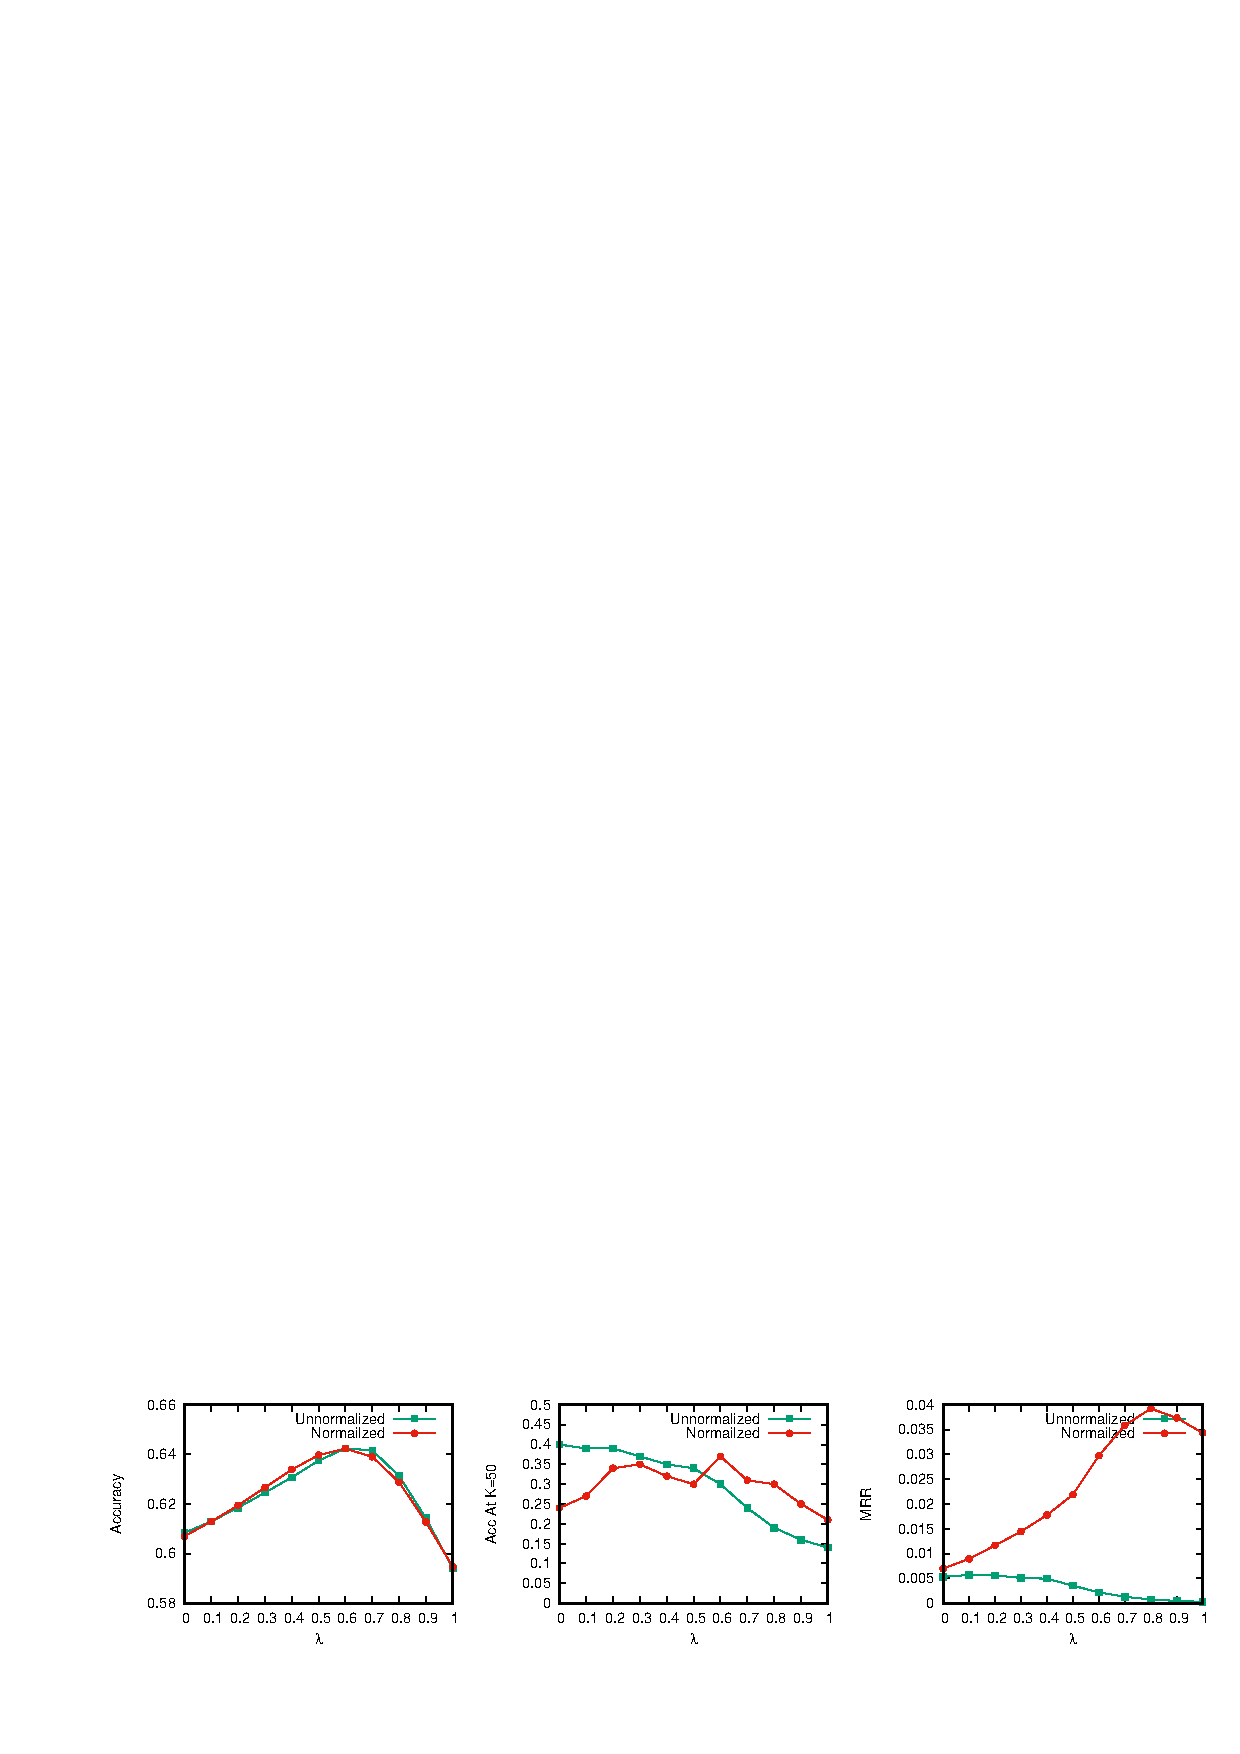
\includegraphics[width=2\columnwidth]{lambda}
	\caption{Evaluation on different $\lambda$s}
	\label{fig:lambda}
\end{figure*}


\paragraph{Span Size}
We define the cause and effect span in Eection~\ref{subsec:vec repre} which are the whole span of the half sentence. However, it is more likely that the real cause or effect appears closer to the causal cue. For sentences in Example~\ref{eg:sen}, key event ``flooding'', ``damage'', ``downpour'' are all within 3 words from the pattern. Proper span size can improve our result by removing irrelevant words but also takes the risk of losing the knowledge. 

\begin{figure*}[th]
	\centering
	%\epsfig{file=causalnet.eps, width=0.6\columnwidth}
	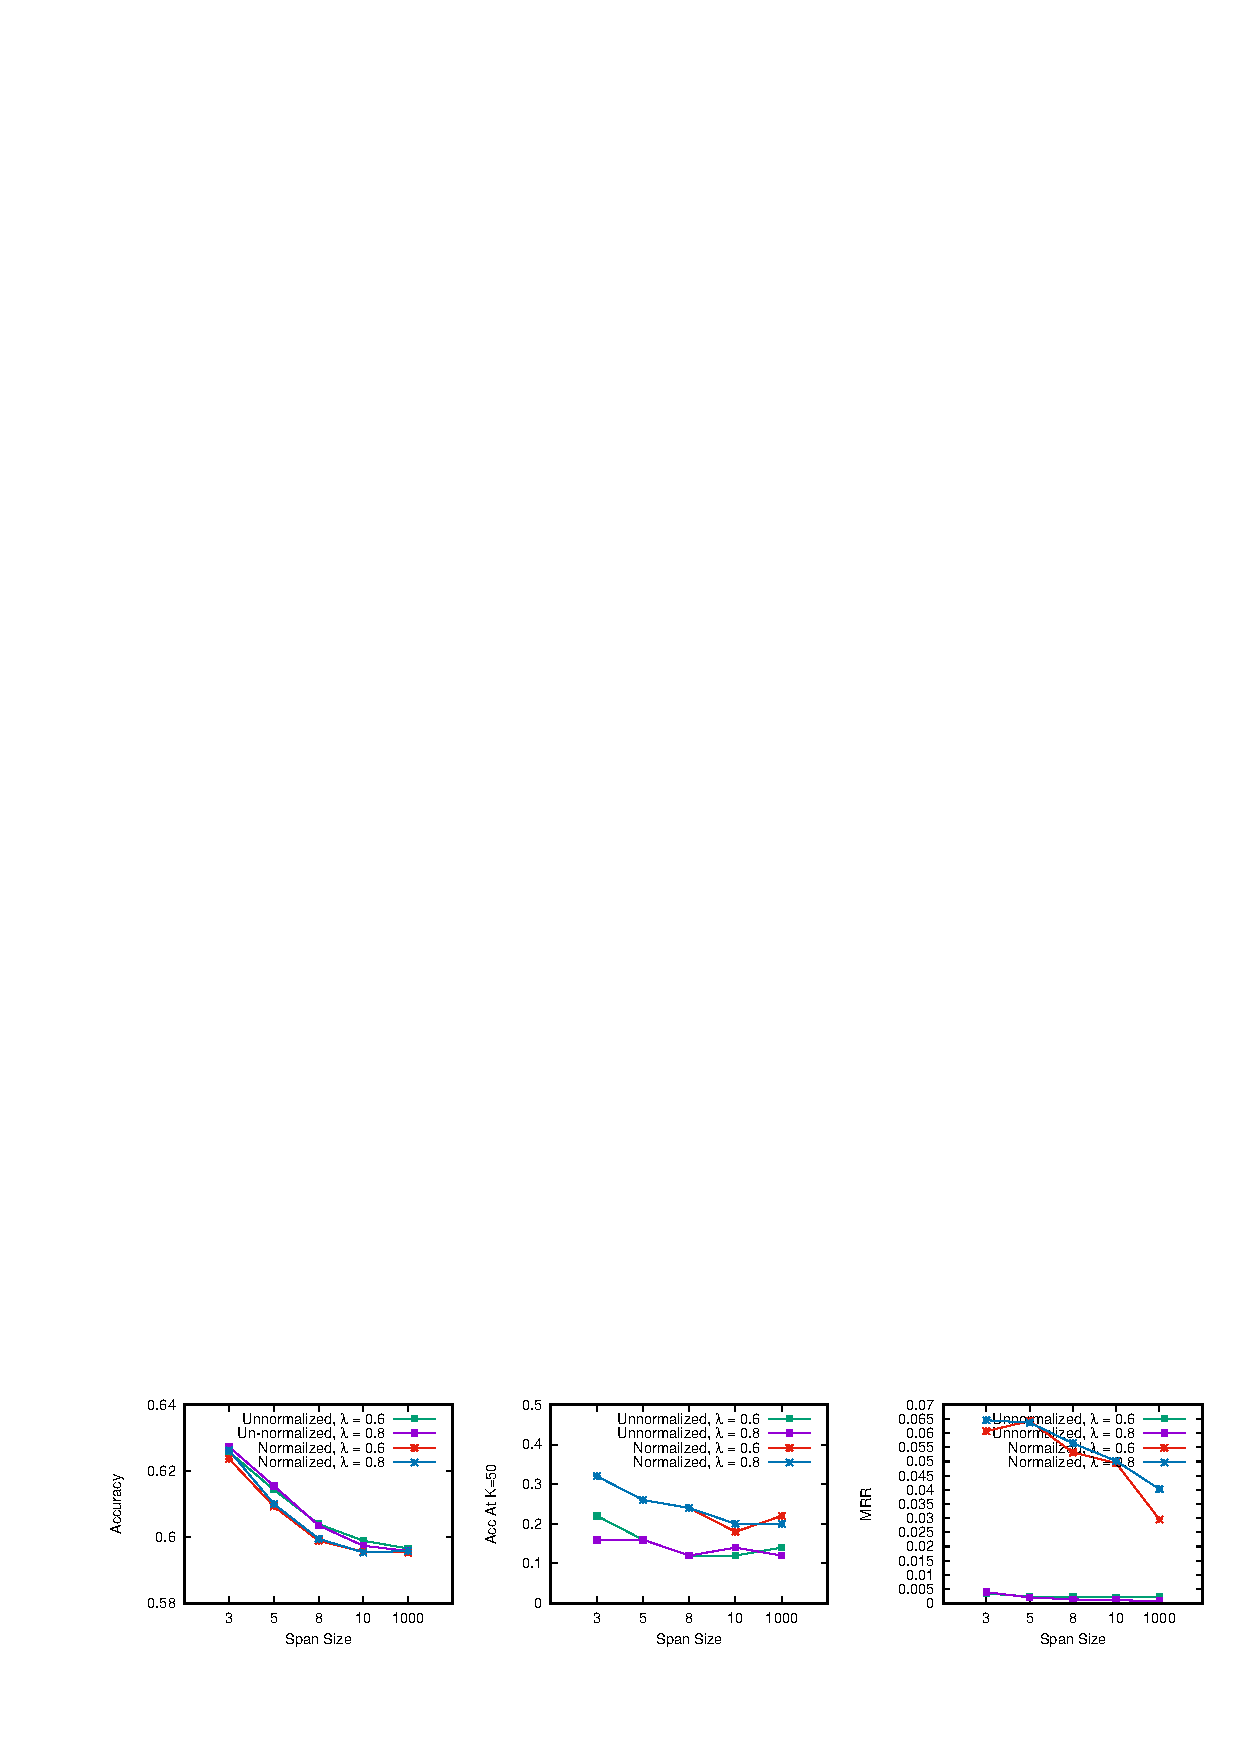
\includegraphics[width=2\columnwidth]{spansize}
	\caption{Evaluation on different span sizes}
	\label{fig:spansize}
\end{figure*}

\paragraph{Iteration Times}
As the iteration number increase, the quality of the dataset gets better. Figure shows ....

\paragraph{Qualitative Result}
\begin{table*}[!ht]
	\caption{Sample of causal pairs}
	\label{tab:qualitative}
	\centering
	\small
		\begin{tabular}{|l|l|l|}
			\hline 
			Cauase & Top Effects of Embedding& Top Effects of Luo et al. \cite{luo2016commonsense} \\
			\hline
			rainfall & flooding, flood, drought& roundheaded, litchee, epipactis\\
			accident & fatality, die, death, fatal& distrait, crippling, aviatrix\\
			virus & hepatitis, infected, viremia&  ecballium, hominoidea, discase\\
			drown & death, swim, suffocation& equaphobia, diminutiveness\\
			pregnant & abortion, fetus, baby&jotunn, pycnanthemum, lopid \\
			\hline 
			\hline
			Effect & Top Causes of Embedding& Top Causes of Luo et al. \cite{luo2016commonsense} \\
			\hline
			damage & magnitude-5, waterspout&reliance, tornade, vehicular\\
			happy & love, joy, wonderful, hope&offend, flag, reproach, goosy\\
			light & illumination, bright, lamp& air, refractive, phototropism\\
			hurt & feel, break, cheat, love& dacoity, screwing, padding\\
			die & complication, accident& complication, accident, sustain\\
			\hline
	\end{tabular}
\end{table*}
We compare our final results with Luo~\cite{luo2016commonsense}'s dataset. The results are shown in Table~\ref{tab:qualitative}.



\subsection{Application}
We apply our causal embeddings on Choice of Plausible Alternatives(COPA)~\cite{roemmele2011choice}, a multiple-choice problems asking for cause or effect given the other side. Below is one example of COPA dataset.

\begin{example}
	\label{ex:copa}
	\noindent
	\begin{itemize}
		\item[] Premise: \emph{I knocked on my neighbor's door.} What
		happened as an effect?
		\item[] Alternative 1: \emph{My neighbor invited me in.}
		\item[] Alternative 2: \emph{My neighbor left her house.}
	\end{itemize}
\end{example}

In this example, we are given the cause side event ``\emph{I knocked on my neighbor's door.}'' and required to choose the more possible effect.
We solve this problem by two sides.

\paragraph{Sentence-level Solution}
Since we already have the word embedding for cause and effect roles, we can generate the sentence embedding for premise and alternative by averaging the sum of all words' vectors.
The causal strength between the two sentences is the dot product of the two vectors.

\begin{equation}
	CS_{sen}(S_1, S_2) = (\frac{1}{|S_1|}\sum_{c_i \in S_1}{\overrightarrow{c_i}}) \cdot (\frac{1}{|S_2|}{\sum_{e_j \in S_2}\overrightarrow{e_j}})
\end{equation}

\paragraph{Word-level Solution}
We can also follow the method used by Luo~\cite{luo2016commonsense}, using the word level causal strength.
\begin{equation}
	CS_{word}(S_1, S_2) = \frac{\sum_{c_i \in S_1, c_j \in S_2}{\overrightarrow{c_i} \cdot \overrightarrow{e_j}}}{|S_1|+|S_2|}
\end{equation}
